\chapter{Image Classification}

\begin{glancebox}
Before a computer can tell a can from a plastic bottle, you must understand what an image is and how to build a good set of examples. This chapter explains images, classification, and how to collect, store and test pictures, using a trash classifier as the running example.
\end{glancebox}

\section*{Learning objectives}

By the end of this chapter you can:


\begin{enumerate}
\item Describe what an image is and name the common image types.
\item Explain image classification and tell binary from multi-class problems.
\item Identify the \emph{input} and \emph{output} of an image classifier.
\item Collect, diversify and store a dataset with one folder per class.
\item Describe how training data, a trained model and test data fit together.
\end{enumerate}

\section*{Key terms}

\textbf{Image} · \textbf{RGB} · \textbf{grayscale} · \textbf{binary image} · \textbf{width and height} · \textbf{image classification} · \textbf{binary classification} · \textbf{multi-class classification} · \textbf{input} · \textbf{output (label)} · \textbf{dataset} · \textbf{diversity} · \textbf{training data} · \textbf{test data}


\section{What is an image?}

A digital \textbf{image} is a grid of tiny dots called pixels. Several types appear in this course and in real life:


\begin{itemize}
\item \textbf{RGB} images store \textbf{R}ed, \textbf{G}reen and \textbf{B}lue values for every pixel, giving full colour.
\item \textbf{Grayscale} images keep only light and dark.
\item \textbf{Binary} images have just two values, black and white.
\item Special images include \textbf{X-rays} (medical scans of the chest, for example) and \textbf{satellite} photos (a city seen from above).
\end{itemize}

Figure \ref{fig:flower-image-types} shows the same flower as an RGB, a grayscale and a binary image.


\begin{figure}[htbp]
\centering
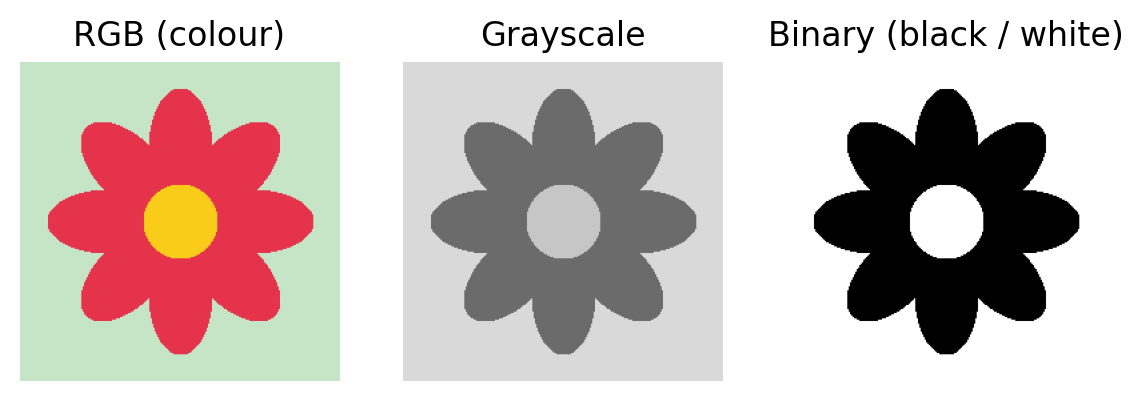
\includegraphics[width=0.9\linewidth]{figures/generated/flower-image-types.png}
\caption{The same flower as an RGB (colour), grayscale and binary image.}\label{fig:flower-image-types}
\end{figure}

\textbf{Image size} is described by \textbf{width} and \textbf{height}. Images can be small, medium or large. A bigger image holds more detail but takes more computing power. (In Chapter 7 you will see that Teachable Machine resizes every webcam frame to 224 \ensuremath{\times} 224 pixels.)


\begin{notebox}
\textbf{Go deeper.} Want to know what a computer really stores for each pixel? See Appendix A, \emph{How Computers See Pictures}.
\end{notebox}

\section{What is image classification?}

\textbf{Image classification} means giving an image a label. In this chapter the labels are kinds of rubbish:


\begin{itemize}
\item \textbf{Binary classification}: only two possible labels, for example \emph{can (metal)} vs. \emph{plastic}.
\item \textbf{Multi-class classification}: three or more labels, for example \emph{can (metal)} vs. \emph{plastic} vs. \emph{paper}.
\end{itemize}

Figure \ref{fig:binary-vs-multiclass} compares the two: with two labels the model must pick one or the other, while with three or more labels it picks one of several.


\begin{figure}[htbp]
\centering
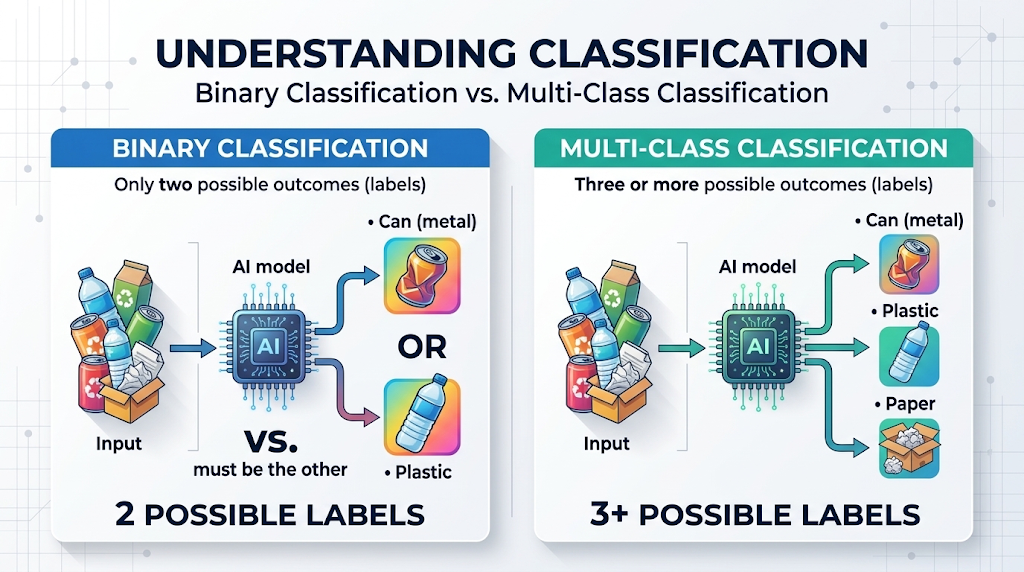
\includegraphics[width=0.95\linewidth]{figures/provided/binary-vs-multiclass.png}
\caption{Understanding classification: binary classification has two possible labels (can or plastic); multi-class classification has three or more (can, plastic or paper).}\label{fig:binary-vs-multiclass}
\end{figure}

\subsection*{The elements of a classifier}

Every image classifier has the same two parts. For a \textbf{trash image classifier}:


\begin{itemize}
\item \textbf{Input}: an image.
\item \textbf{Output}: a label (Plastic, Can or Paper).
\end{itemize}

Figure \ref{fig:trash-classifier} shows the input and output of the trash classifier.


\begin{figure}[htbp]
\centering
\adjustbox{max width=\linewidth}{\begin{tikzpicture}[x=1cm,y=1cm]
\node[box,minimum width=2.6cm] (img) at (0,0) {\textbf{Input}\\[-1pt]{\scriptsize an image}};
\node[box,minimum width=3.2cm,fill=blue!10] (mod) at (4.6,0) {\textbf{Trash classifier}\\[-1pt]{\scriptsize AI model}};
\draw[arrow] (img)--(mod);
\foreach \y/\t/\c/\n in {1.4/Can (metal)/gray!35/oa, 0/Plastic/blue!25/ob, -1.4/Paper/green!25/oc}{
 \node[draw,rounded corners=2pt,fill=\c,minimum width=2.6cm,minimum height=0.9cm] (\n) at (9.4,\y) {\textbf{\t}};
 \draw[arrow] (mod.east)--(\n.west);}
\node[font=\scriptsize] at (9.4,2.3) {\textbf{Output: a label}};
\end{tikzpicture}
}
\caption{A trash image classifier: an image goes in and a label comes out.}\label{fig:trash-classifier}
\end{figure}

\subsection*{Why classify images?}

Sorting rubbish for recycling is one reason; the same idea reaches medicine (X-rays), farming, traffic signs and satellites. \textbf{Think about it:} list other cases of image classification in your own community.


\section{Collecting data}

A model can only learn from what you show it, so data collection is the most important step.


\subsection*{Where do pictures come from?}

\begin{itemize}
\item a \textbf{camera},
\item a \textbf{mobile phone},
\item a \textbf{webcam},
\item \textbf{Google Image Search}.
\end{itemize}

\subsection*{Diversity of data}

Do not take ten photos of the same can. Collect \emph{different} cans, \emph{different} plastics and \emph{different} papers. Vary the angle, the light and the background. If every can in your set is the same brand, the model may only learn that brand.


Figure \ref{fig:diversity-of-data} contrasts the two approaches: ten photos of the same can teach the model only one brand, while different items, angles, lighting and backgrounds teach it what a can, a plastic bottle and paper really look like.


\begin{figure}[htbp]
\centering
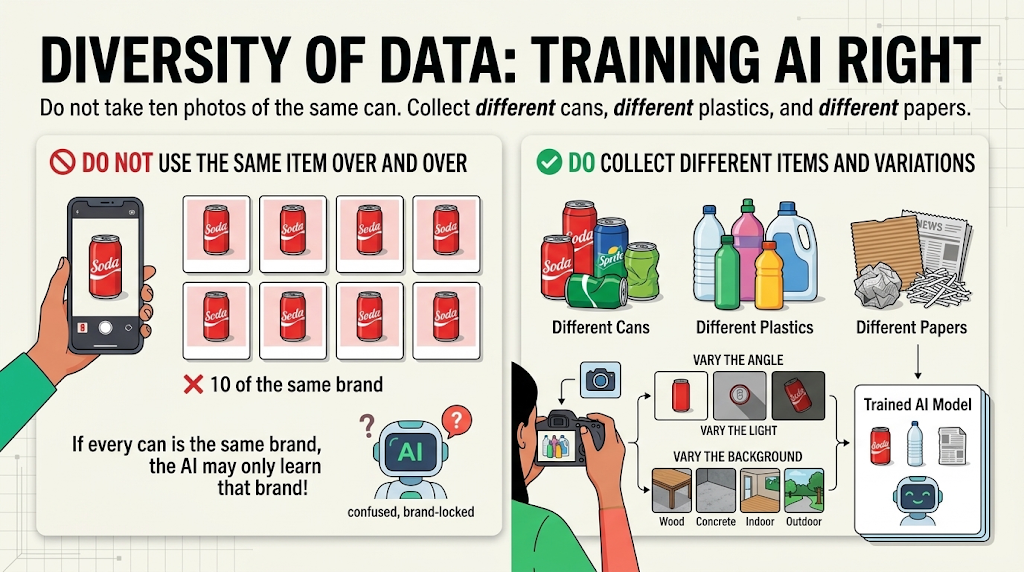
\includegraphics[width=0.95\linewidth]{figures/provided/diversity-of-data.png}
\caption{Diversity of data: do not use the same item over and over; collect different items and vary the angle, the light and the background.}\label{fig:diversity-of-data}
\end{figure}

\subsection*{Storing your data}

Keep one \textbf{folder per class}:


\begin{itemize}
\item \texttt{Can (metal)} folder
\item \texttt{Plastic} folder
\item \texttt{Paper} folder
\end{itemize}

Figure \ref{fig:folder-structure} shows how one folder per class keeps the dataset organized.


\begin{figure}[htbp]
\centering
\adjustbox{max width=\linewidth}{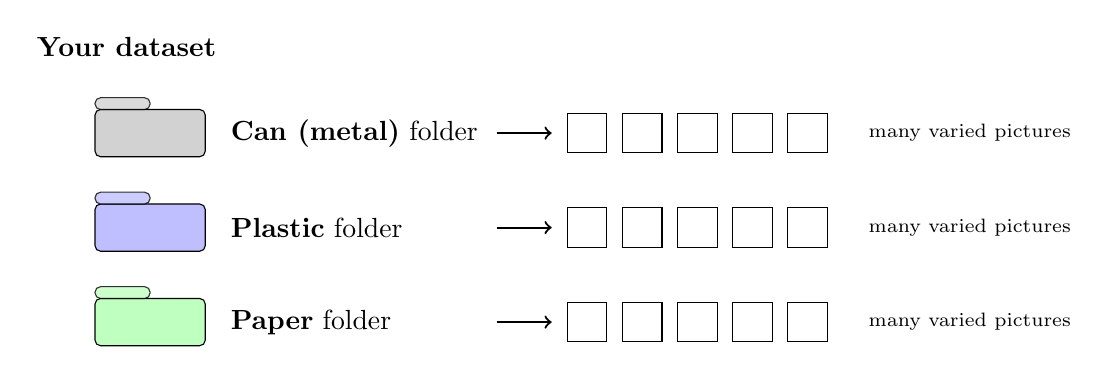
\begin{tikzpicture}[x=1cm,y=1cm]
\node[font=\bfseries] at (0,2.3) {Your dataset};
\foreach \y/\n/\c in {1.2/Can (metal)/gray!35, 0/Plastic/blue!25, -1.2/Paper/green!25}{
 \draw[fill=\c,rounded corners=2pt] (-0.4,\y-0.3) rectangle (1.0,\y+0.3);
 \draw[fill=\c,opacity=0.8,rounded corners=2pt] (-0.4,\y+0.3) rectangle (0.3,\y+0.45);
 \node[anchor=west] at (1.2,\y) {\textbf{\n} folder};
 \foreach \k in {0,1,2,3,4}{\draw[fill=white] (5.6+\k*0.7,\y-0.25) rectangle (6.1+\k*0.7,\y+0.25);}
 \node[anchor=west,font=\scriptsize] at (9.3,\y) {many varied pictures};
}
\draw[thick,->] (4.7,1.2)--(5.4,1.2); \draw[thick,->] (4.7,0)--(5.4,0); \draw[thick,->] (4.7,-1.2)--(5.4,-1.2);
\end{tikzpicture}
}
\caption{One folder per class keeps the dataset organized.}\label{fig:folder-structure}
\end{figure}

Putting a picture in the wrong folder gives the model a wrong lesson, so check carefully.


\section{Training and testing with Teachable Machine}

\begin{enumerate}
\item \textbf{Training data.} The folders of pictures go into \href{https://teachablemachine.withgoogle.com}{Google Teachable Machine}. Each folder becomes a class.
\item \textbf{Training.} Teachable Machine learns from the folders and produces the \textbf{trash classifier model}.
\item \textbf{Test data.} Show the model \emph{new} pictures it has not seen. It answers CAN, PAPER or PLASTIC.
\end{enumerate}

Always test with pictures that were not in the training folders, otherwise you are only checking its memory, not its learning.


\textbf{A trained model for reference.} A finished version of the trash classifier is online. Open it, allow the camera if asked, and test it with items from your own bag or classroom: \href{https://teachablemachine.withgoogle.com/models/2i97CAy5C/}{https://teachablemachine.withgoogle.com/models/2i97CAy5C/}. It is an Image model with three classes, \emph{Plastic}, \emph{Metal} and \emph{Paper}. (Its “Metal” class plays the role of the “Can” class in this chapter.) Try the hard cases from Section 2.5 and see where it fails.


\section{Hard test cases}

Real life is messier than your training set. Good test pictures include a \textbf{dented can}, a \textbf{newspaper advertisement page} (paper, but colourful and full of text) and a \textbf{clear plastic item against a wall}. If the model struggles with these, add more varied examples of that class and train again. (Chapter 3 shows how.)


\section{Practice time}

Build the trash classifier, or the classifier you sketched in Chapter 1:


\begin{enumerate}
\item Decide on 2–3 classes.
\item Collect a varied set of pictures for each class.
\item Store each class in its own folder (or add them directly in Teachable Machine).
\item Train, then test with new pictures, including a few hard ones.
\end{enumerate}

\section*{Summary}

\begin{itemize}
\item An image is a grid of pixels; common types are RGB, grayscale and binary.
\item Classification gives an image a label; it is binary with two labels and multi-class with three or more.
\item A classifier takes an image as input and outputs a label.
\item Good data is varied, correctly labeled and stored one folder per class.
\item Always test with pictures the model has never seen.
\end{itemize}

\section*{Check your understanding}

\begin{enumerate}
\item Is “cat / dog / rabbit” binary or multi-class? Why?
\item Name three ways to get pictures for a dataset.
\item Why is it a bad idea to take all your “can” photos of one brand?
\item Why should test pictures be different from training pictures?
\end{enumerate}

\emph{Answer hints:} (1) multi-class (three labels). (3) The model may learn the brand, not “can”. (4) To measure learning, not memory.


\section*{Further practice}

Find a classification problem in your own community that could be solved with pictures. Write its input, its output labels and where you would collect the data.


\medskip\noindent\hrulefill\medskip
